\documentclass[3p]{article}
\usepackage[latin1]{inputenc}
\usepackage{amsmath}
\usepackage{fixmath}
\usepackage{amssymb}
\usepackage{graphics}
\usepackage{breqn}
\usepackage{algorithmicx}
\usepackage[ruled]{algorithm}
\usepackage[noend]{algpseudocode}
\usepackage{titlesec}
\usepackage{graphicx}
\usepackage{subfigure}
\usepackage{tabto}
\usepackage{hyperref}
\hypersetup{
    colorlinks=true,
    linkcolor=blue,
    filecolor=blue,      
    urlcolor=blue,
    citecolor=blue,
}

\begin{document}

\title { POD-XIgA: A 1D Numerical Example}
\author{Massimo Carraturo}

\maketitle

%%%%%%%%%%%%%%%%%%%%%%%%%%%%%%%%%%%%%%%%%%%%%%%%%%%%%%%%%%%%%%%%%%%%%%%%%%%%%%%%%%%%%%%%%%%%%%%%%%%%%%%%%%%%%%%%%%%
% INTRODUCTION

\section*{Introduction}
AM processes are gaining an increasing importance in many engineering fields, from mechanical to civil engineering applications. In particular in the recent years the 3D printing technology has known an exponential growth and it has been applied to produce a wide range of products.
Nevertheless, the simulation of an AM process still presents several computational issues due to the high complexity of the underlying physical problem. In particular, this kind of problem turns out to be:
\begin{itemize}
\item \textit{Transient}: the high speed of the laser beam does not allow to neglect the thermal inertia of the material.
\item \textit{Non-linear}: due to the broad range of temperatures involved, both the heat capacity and the conductivity depends on the temperature.
\item \textit{Multi-Phase}: three different phase of the material have to be considered: powder, liquid and solid.
\item \textit{Multi-Scale}: the dimension of the laser beam is order of magnitude smaller than the size of the problem domain.
\end{itemize}
The high number of computational challenges involved calls for more sophisticated methods: Reduced Order Model (ROM) seems to be a promising direction \cite{Rozza2009}.
\\
\\
\indent ROM can be efficiently applied in the context of AM. In facts, this technique allows to speed-up the overall computational time, when several evaluation of the same problem has to be computed varying one or more parameters. There are no restrictions on the nature of the parameters which can be varied, they can include: the laser power, the laser beam size as well as the boundary conditions at different positions along the laser path.
In the literature the ROM was already applied to heat transfer problems by means of different techniques:
\begin{enumerate}
\item Classical Model Reduction: The full order model (FOM) is first solved for a small number of different parameter values (training-phase). From the set of FOM solutions (\textit{snapshots}) a reduction operator is constructed using the proper orthogonal decomposition (POD). The analysis is then performed on the ROM, which is obtained simply projecting the discrete system onto the reduced space by means of the reduction operator (ROM-phase) \cite{Michopoulos2014a}.
The main drawback of this method is that computational speed-up affect only the time required to solve the system, while the integration still has to be performed on the full model.
\item {POD-GFEM} \cite{Aquino2008}: In this method the POD modes extracted from the set of snapshots are used to enriched the FEM basis via partition of unity \cite{Babuska1997} approach (GFEM/XFEM). The POD-GFEM allows to integrate and solve the problem on a coarse mesh enriched using POD modes. With this method high accuracy can be achived with a relatively small number of DOFs.
\item {V-GFEM}: The \textit{Vademecum}-GFEM \cite{Canales2016a} uses a different decomposition method: the so called proper generalized decomposition (PGD). This method allows to generate the solution snapshots on a local domain with an eulerian reference frame. The PGD results are again used to enrich the FEM basis following the GFEM approach. The two main advantages of this method are the reduced number of additional DOFs and the local/global feature of the method itself, since the \textit{Vademecum} is generated separately on a local domain and allows to enrich only the nodes around the heat affected zone (HAZ).
\end{enumerate}

%%%%%%%%%%%%%%%%%%%%%%%%%%%%%%%%%%%%%%%%%%%%%%%%%%%%%%%%%%%%%%%%%%%%%%%%%%%%%%%%%%%%%%%%%%%%%%%%%%%%%%%%%%%%%%%%%%%
% X-PODFEM

\section*{POD-XIgA}

In the present work we seek for a method which first allows to capture with a relatively low number of DOFs the non-linear behaviour of an AM process and secondly leads to a considerable computational speed-up. Another objective is to avoid the separation of the training and the ROM-phase. POD-XIgA approach exploits the local/global feature required in AM applications and allows to take advantage from the higher approximation property of Isogeometric analysis (IgA) \cite{cottrell_isogeometric_2009}.

%%%%%%%%%%%%%%%%%%%%%%%%%%%%%%%%%%%%%%%%%%%%%%%%%%%%%%%%%%%%%%%%%%%%%%%%%%%%%%%%%%%%%%%%%%%%%%%%%%%%%%%%%%%%%%%%%%%
% POD

\subsection*{POD}
There are many different techniques which allow to generate reduced basis functions. One of the most popular is the \textit{Proper Orthogonal Decomposition} also called \textit{Karhunen-Lo{\'e}ve decomposition} or \textit{Galerkin projection}, an explore-and-compress method. The parameter space is investIgAted generating some randomly-distributed sample points (or \textit{snapshots}), i.e. the true solution at a given parameter value. Then the method compress the continuous parameter space into a reduced one, filtering only the information which are essential to approximate the true solution space, i.e. the modes corresponding to the higher energetic eigenvalues. This randomness in the snapshots generation makes the POD particularly suitable to capture the casualty associated with the time evolution of the process. The POD can be also defined as a method for constructing lower-dimensional approximation of a subspace in Hilbert space, as the \textit{Single Value Decomposition} (SVD) does in a finite-dimensional space or Euclidean space.\\Given a set of \textit{M-snapshots} 
\begin{equation}
\mathcal{M}(\mathbb{P}_{h}) = \lbrace\theta(\mu)\vert\mu \in \mathbb{P}_{h}\rbrace
\end{equation}
where $\mathbb{P}_{h} \subset \mathbb{P}$ is a discrete point-set in the parameter domain and $\theta(\mu)$ the solution vector at a give $\mu$. Let $\mathbf{T}$ being the matrix whose columns are the solution vector at each snapshot, we define the \textit{solution covariance matrix} $\mathbf{Y}$ as
\begin{equation}
\mathbf{Y} = \mathbf{T}^{T} \times \mathbf{T}.
\label{eq:covarianceMatrix}
\end{equation}
The $N_{RB}$-dimensional ( where $N_{RB} < M$ is the number of eigenvalues of $\mathbf{Y}$ higher than a given tolerance) POD-space is given by the set of orthonormal vectors $\lbrace \zeta_{i} \rbrace_{i=1}^{N_{RB}} \subset \mathbb{R}^{N_{RB}}$ which solve the minimization problem \\
\indent
\begin{equation}
\min_{\lbrace\zeta_{i}\rbrace_{i=1}^{N_{RB}}}\sum_{j=1}^{M} 
\| \mathbold{\theta}_{j}(\mu) - \sum_{i=1}^{N_{RB}}(\mathbold{\theta}_{j}^{T}(\mu)\zeta_{i})\zeta_i\|_{\mathbb{V}}^{2}
\label{eq:minPOD}
\end{equation}
where $\Vert\cdot\Vert_{\mathbb{V}}$ is the norm induced by the parametrized bilinear form (we refer to \cite{Rozza2009} for further details) for a given $\mu$
\begin{equation}
\Vert\cdot\Vert_{\mathbb{V}} = \sqrt{\mathcal{B}(\cdot, \cdot; \mu)}
\end{equation}
and with
\begin{equation}
\zeta_{i}^{T}\zeta_{j} = \delta_{ij} =
    \begin{cases}
      1 &\text{if}\quad i=j, \\
      0 &\text{if}\quad i \neq j, \\
    \end{cases}
   \quad i,j=1,...,N_{RB}.
\end{equation}
\indent Algorithm \ref{PODAlg} gives a solution for (\ref{eq:minPOD}), starting from the eigendecomposition of the snapshots covariance matrix $\mathbf{Y}$, a normalized set of column vectors $\mathbf{\bar{U}}$ is derived allowing to transform the shape functions $\phi_{k}$ used to approximate the full problem into a set of reduced basis $\zeta_{i}$. 
\begin{algorithm}
\caption{POD}
\begin{algorithmic}[1]
\State \textit{input}: $\Theta_{i j}(\mu) \quad M\times N $\textit{snapshots}-matrix and $\phi_{i}$ vector of FOM-basis functions.
\State \textit{output}: $\zeta_{i}$ $N_{RB}-$reduced basis functions.
\State $Y_{ik}=\Theta_{ij}(\mu)\Theta_{jk}(\mu)$ 
\State $SVD(Y_{ik})=\nu_{ik}\lambda_{kk}\nu_{ki}$
\If {$\lambda_{kk} \geq tolerance$}
\State $sort(\lambda_{kk}, \nu_{ik})$
\EndIf
\State $U_{ki}=\dfrac{1}{\sqrt{\lambda_{kk}}}\sum_{j=1}^{N_{RB}}\nu_{ij}\Theta_{ik}(\mu)$ 
\State $\bar{U}_{ki}=\dfrac{U_{ki}}{\Vert U_{ki}\Vert}$ 
\State $\zeta_{i}=\phi_{k}\bar{U}_{ki}$.
\end{algorithmic}
\label{PODAlg}
\end{algorithm}

%%%%%%%%%%%%%%%%%%%%%%%%%%%%%%%%%%%%%%%%%%%%%%%%%%%%%%%%%%%%%%%%%%%%%%%%%%%%%%%%%%%%%%%%%%%%%%%%%%%%%%%%%%%%%%%%%%%
% PARTITION OF UNITY

\subsection*{Partition of Unity (PU) expansion}
The set of reduced basis $\zeta_{i}$ obtained from POD (\textit{aka} POD-modes) can be used to enrich the initial set of shape functions $\phi_{k}$ via the partition of unity expansion \cite{Babuska1997}
\begin{equation}
\theta_{h}(x) = \sum_{i\in I} \phi_{i}(x)\theta_{i} + \sum_{\alpha}\sum_{j\in I_{enr}} \phi_{j}(x)\zeta_{\alpha}a_{j\alpha}
\label{PartitionOfUnity}
\end{equation}
where $I$ is the set of all nodes of the initial (coarse) discretization, $\alpha$ is the number of considered POD-modes and $I_{enr}$ is the set of nodes enriched by means of POD-modes. This enrichment of standard basis can be performed only if the shape functions $\phi_{k}$ satisfies the partition of unity, i.e. $\sum_{k=1}^{n}\phi_{k}(x)=1$. The POD-modes represents the general behaviour of the solution, thus, if they are used as enrichment functions, allow to capture the main solution features using a relatively relatively small number of DOFs. It is clear that the construction of the POD-modes, i.e. the training-phase, plays a vital role in this methodology. As aforementioned, one objective of the present method is to integrate in the same simulation process the training and the ROM-phase and at the same time, enrich only the DOFs within the region of interest. To achieve such a goal the training-phase is made "\textit{on-fly}":
\begin{enumerate}
\item The FOM simulation employs a fine mesh to solve the partial differential equations (PDE), which describe the problem.
\item POD is performed on the temperature solutions around the HAZ cached during the training phase.
\item In the ROM phase a coarse mesh is used to solve the global problem, such a mesh is locally enriched around the HAZ.
\end{enumerate}

%%%%%%%%%%%%%%%%%%%%%%%%%%%%%%%%%%%%%%%%%%%%%%%%%%%%%%%%%%%%%%%%%%%%%%%%%%%%%%%%%%%%%%%%%%%%%%%%%%%%%%%%%%%%%%%%%%%
% IgA

\subsection*{Isogeometric analysis}
Isogeometric analysis represents a novel technique which aims to integrate Computer Aided Design(CAD) and numerical analysis. This goal is achieved employing the CAD-standard technology of Non-Uniform Rational B-spline (NURBS) as set of function for the analysis. The first consequence of this approach is that complex geometries can be represented exactly. NURBS also allow to arbitrary increase the inter-element continuity, leading to a more precise representation of derivatives of the field variables. Finally, higher order Ansatz spaces generated using NURBS capture complex solution with a lower number of DOFs than standard FEM techniques.
In the present work B-splines are used as basis for the analysis. In fact, these curves are easier to deal with in numerical analysis and at the same time carry over all the key features of NURBS.
\subsubsection*{B-spline basis functions}
B-splines are curves based on parametric functions, i.e. they represent a given geometry by means of parameters. The physical (geometric) space has to be mapped onto a parametric space where the parametric function is defined. In particular, to construct a B-spline a \textit{knot vector} $\Xi=\left\lbrace\xi_{1},\xi_{2},...,\xi_{n+p+1}\right\rbrace$, where $\xi_{i} \in \mathbb{R}$ is the $i^{th} knot$, $i$ is the knot index, $p$ is the polynomial order and $n$ is the number of basis functions used to constructed the curve, must be specified. The knot vector in one-dimension is a non-decreasing set of coordinates in the parameter space. The knots partition the parameter space into elements, the so-called \textit{knot-span}. Geometric boundaries in the physical space are the projection of knot lines via the B-spline mapping.
The B-spline mapping can be constructed using the \textbf{Cox-de Boor recursion formula}, where B-spline basis are defined starting with piecewise constants ($p=0$):
\begin{equation}
N_{i,0}(\xi)= 
\begin{cases}
      1, & \text{if}\ \xi_{i} \leqslant \xi < \xi_{i+1} \\
      0, & \text{otherwise}.
\end{cases}
\end{equation}
For $p=1,2,3,...,$ they are defined by
\begin{equation}
N_{i,p}(\xi) = \dfrac{\xi-\xi_{i}}{\xi_{i+p}-\xi_{i}}N_{i,p-1}(\xi)+\dfrac{\xi_{i+p+1}-\xi}{\xi_{i+p+1}-\xi_{i+1}}N_{i+1,p-1}(\xi).
\end{equation}
The second key ingredient for constructing a B-spline curve are \textbf{\textit{control points}}, the vector-valued coefficients of the B-spline basis. Thus, given $n$ basis $N_{i,p}$ and corresponding control points $\mathbf{B_{i}}\in\mathbb{R}$ a B-spline curve is defined by:
\begin{equation}
\mathbf{C}(\xi) = \sum_{i=1}^{n}N_{i,p}(\xi)\mathbf{B}_{i}.
\end{equation}
\subsubsection*{eXtended Isogeometric analysis (XIgA)}
Using B-spline as basis for the analysis do not affect the possibility to enrich the Ansatz space via PU techniques. In fact, one property of the B-spline is that the fulfil the partition of unity, then they can be enriched using the POD-modes extracted from the training phase. The only difference with respect to the classical XFEM enrichment is that using IgA we have to enrich the DOF associated with a control point, which is in general non-interpolatory. Eq. \ref{PartitionOfUnity} reads now:
\begin{equation}
\theta_{h}(x) = \sum_{i\in I} N_{i,p}(x)\theta_{i} + \sum_{\alpha}\sum_{j\in I_{enr}} N_{j,p}(x)\zeta_{\alpha}a_{j\alpha},
\label{IgAPartitionOfUnity}
\end{equation}
which is the numerical approximation of the so-called eXtended Isogeometric analysis (XIgA) using POD-modes as enrichment functions.\\
\\
\indent 
The use of XIgA enriched by means of POD-modes requires additional mapping for the integration of the extended term in Eq. \ref{IgAPartitionOfUnity}. In fact, from Algorithm \ref{PODAlg} we obtain a set of vectors $\zeta_{i}$ of $n$ coefficients. To generate a POD basis which can be integrated using gaussian quadrature the coefficients have to be interpolated using linear functions, such that
\begin{equation}
\zeta_{\alpha}^{h}(x) = \sum_{i}\phi(x)\hat{\zeta}_{i\alpha}.
\end{equation} 
The interpolation functions $\phi(x)$ are defined on a sub-domain $\bar{\Omega}$ of the integration space $\tilde{\Omega}$, therefore an additional affine mapping $\bar{\sigma}:\bar{\Omega}^{el}\rightarrow\tilde{\Omega}^{sel}$ as shown in Figure \ref{fig:IntegrationMappingPODXIgA}.
\begin{figure}
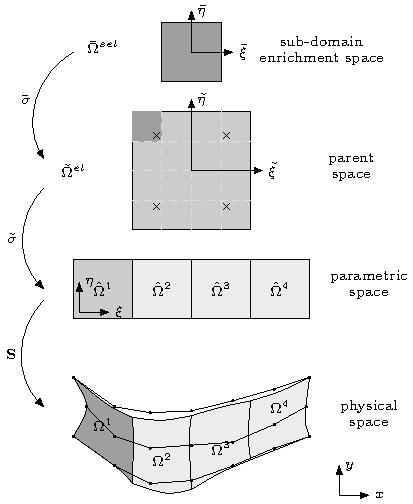
\includegraphics[width=1\linewidth]{externals/Pictures/IntegrationXPOD.pdf}
\caption{Integration is performed by Gaussian quadrature on the parent space. The value of the POD-modes at each Gauss point is obtained by linear approximation of POD-mode coefficients. The set of POD-mode coefficients define a grid called sub-domain enrichment space and the interpolation linear basis are defined on such a space.}
\label{fig:IntegrationMappingPODXIgA}
\end{figure}


%%%%%%%%%%%%%%%%%%%%%%%%%%%%%%%%%%%%%%%%%%%%%%%%%%%%%%%%%%%%%%%%%%%%%%%%%%%%%%%%%%%%%%%%%%%%%%%%%%%%%%%%%%%%%%%%%%%
% NUMERICAL RESULTS

\section*{1D Numerical Example}
As benchmark to test the method presented so far, we use an AM process where a bar having length $0.5$ mm, width $0.5$ mm and height $10$ mm (see Figure \ref{fig:AMBar1D}) is constructed. The process parameter values and the laser characteristics are reported in Table \ref{table::processParameters} and \ref{table::laserParameters}, respectively. The process is modelled using a 1D bar and discretized with an initial coarse mesh, where each element corresponds to a layer of the bar. In the present work the collections of \textit{snapshots} solutions is obtained computing the last layer of the FOM with a mesh refined using a standard $h$-refinement (see Figure \ref{fig:XPODFEMProcess}). In such a way, at each time step of the training-phase the number of snapshot solution coefficients is constant (as required by POD). From these set of snapshots the POD modal basis are generated and later used as enrichment functions to enrich the last node of the coarse mesh in the ROM-phase. 
\\ \indent Figure \ref{fig:1DProcessLayer} shows the evolution of the 1D bar over an interval corresponding to a single layer construction time. In this picture we can observe that the temperature at the lower end of the bar is kept constant. In contrast, the Dirichlet boundary condition at the upper end of the bar is applied only in the melting interval ($\Delta T_{laser}$), while no boundaries are applied during the cooling time ($\Delta T_{cooling}$). With respect to time, each layer time interval is discretized using 10 time steps: 4 for $\Delta T_{laser}$ and 6 for $\Delta T_{cooling}$. \\ In the following we consider three different problems:
\begin{itemize}
\item linear transient heat problem
\item non-linear transient heat problem
\item non-linear transient heat problem with phase change
\end{itemize}

\begin{figure}[!h]
\centering
  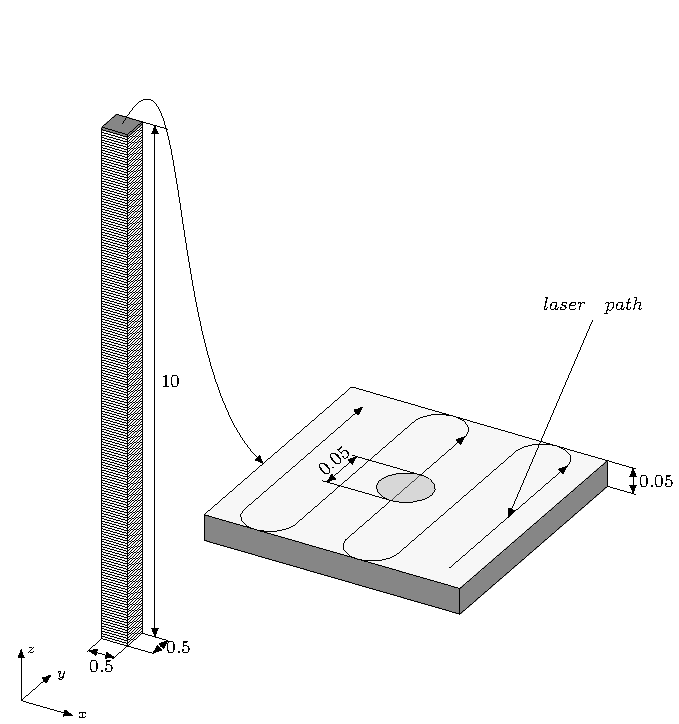
\includegraphics[width=0.8\linewidth]{externals/Pictures/AMBar1D.pdf}
  \caption{AM process of a bar}
  \label{fig:AMBar1D}
  
\end{figure}

\begin{figure}[!h]

  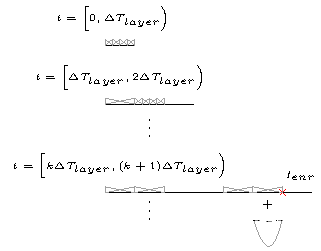
\includegraphics[width=\linewidth]{externals/Pictures/OneDimensionalModelProcess.pdf}
  
 \caption{X-PODFEM learning process: The solution snapshots are generated in the training-phase, which corresponds to the $k$ first layers. In the ROM-phase the last node of the original (coarse) mesh is enriched using POD modes via PU expansion. $\Delta T_{layer}$ is time required to build a single layer of the bar.}
  
  \label{fig:XPODFEMProcess}
  
\end{figure}

\begin{table}[!h]
\centering
    \begin{tabular}{ | l | l | l | p{5cm} |}
    \hline
    number of layers & $10$\\ \hline
    total construction time & $4.5$ $sec$\\ \hline
    laser path length & $0.5$ $mm$\\  \hline
    laser time ($\Delta T_{laser}$) & $0.18$ $sec$\\  \hline
    cooling time ($\Delta T_{cooling}$) & $0.27$ $sec$\\  \hline
    total time per layer ($\Delta T_{layer}$) & $0.45$ $sec$\\  
    \hline
    \end{tabular}
\caption{Bar parameters}
\label{table::processParameters}
\end{table}

\begin{table}[!h]
\centering
    \begin{tabular}{ | l | l | l | p{5cm} |}
    \hline
    laser speed & $2.78$ ${mm}/{sec}$\\ \hline
    initial temperature & $20^{\circ}C$\\ \hline
    laser temperature & $1520^{\circ}C$\\ 
    \hline
    \end{tabular}
\caption{Laser parameters}
\label{table::laserParameters}
\end{table}



%%%%%%%%%%%%%%%%%%%%%%%%%%%%%%%%%%%%%%%%%%%%%%%%%%%%%%%%%%%%%%%%%%%%%%%%%%%%%%%%%%%%%%%%%%%%%%%%%%%%%%%%%%%%%%%%%%%
% LINEAR

\subsection*{Linear transient heat problem}
\begin{figure}[!h]
\centering
  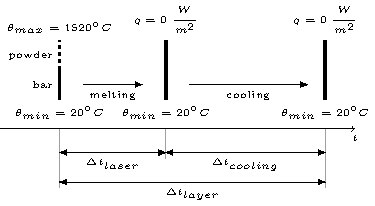
\includegraphics[width=0.8\linewidth]{externals/Pictures/OneDimensionalPhysicalModelProcess.pdf}
  \caption{Single layer time evolution process}
  \label{fig:1DProcessLayer}
  
\end{figure}
\begin{figure}[!h]
\centering
  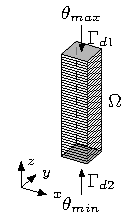
\includegraphics[width=0.4\linewidth]{externals/Pictures/AMBar1DInProgress_mod.pdf}
  \caption{Bar problem}
  \label{fig:1DProblem}
  
\end{figure}
First we want to evaluate the method for a simple linear case where all the physical parameters of the problem are independent of the temperature.
The problem depicted in Figure \ref{fig:1DProblem} is described by the heat transfer partial differential equation (PDE):
\begin{equation}
\rho c \dfrac{\partial\theta}{\partial t} - \kappa\dfrac{\partial\theta}{\partial x} = 0 \qquad \text{on} \quad \Omega,
\end{equation}
with boundary conditions:
\begin{equation}
	\theta = \theta_{min} \qquad \text{on} \quad \Gamma_{d2}
\end{equation}
and
\begin{equation}
	\theta = \theta_{max} \qquad \text{on} \quad \Gamma_{d1} \quad \text{if} \quad T \in \Delta T_{laser},
\end{equation}
with density $\rho = 7500 \dfrac{kg}{m^{3}}$, specific heat $c = 600 \dfrac{J}{kg^{\circ}C}$ and thermal conductivity $\kappa = 27.0 \dfrac{W}{m K}$.
Figure \ref{fig:LinearConvergenceStudy} shows the relative error in the energy norm after 20 layer. In the X-PODFEM the training phase comprises the first 10 layers, $m$ is number of POD-modes and the enriched function is integrated using $m+1$, $m+5$ and $m+10$ Gauss integration points, respectively. In the FEM curve $depth$ indicates the $h$-refinement depth of the last element of the mesh, i.e. the last element is refined using $2^{depth}$ elements. The reference solution is obtained using FEM with $depth=8$. It can be noticed that the results for a single mode are independent of the number of quadrature points used in the integration. Contrary, if we use more then one mode, over-integration is needed to correctly integrate the enriched shape function. The computational speed-up factor obtained using X-PODFEM (for the same level of accuracy) is approximatively 8.8 (see Figure \ref{fig:TimeLinearComparison}) .

\begin{figure}[!h]
\centering
  \subfigure[Convergence study of the linear problem.]  {\label{fig:LinearConvergenceStudy} 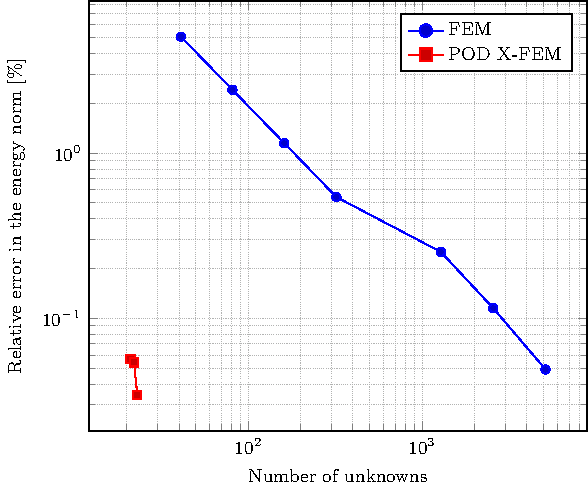
\includegraphics[width=0.75\linewidth]{externals/pgfplots/XFEMLinearConvergenceStudy.pdf}}
  \subfigure[Time comparison FEM vs X-PODFEM.]  {\label{fig:TimeLinearComparison} 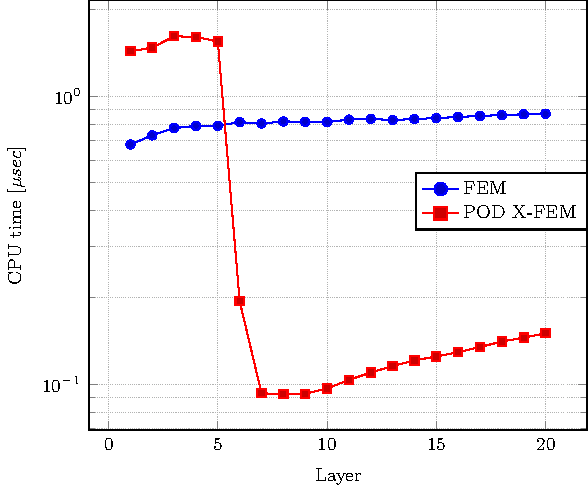
\includegraphics[width=0.5\linewidth]{externals/pgfplots/XFEMLinearTimeResults.pdf}}
  \caption{Linear problem results}
  \label{Linear}
\end{figure}

%%%%%%%%%%%%%%%%%%%%%%%%%%%%%%%%%%%%%%%%%%%%%%%%%%%%%%%%%%%%%%%%%%%%%%%%%%%%%%%%%%%%%%%%%%%%%%%%%%%%%%%%%%%%%%%%%%%%%%%%%%%%%%%%%%%%%%
% NON-LINEAR

\subsection*{Non-linear transient heat problem}
Isogemetric analysis (IgA)\cite{cottrell_isogeometric_2009}


\begin{figure}[!h]
\centering
  \subfigure[Convergence study of the non-linear problem.]  {\label{fig:NonLinearConvergenceStudy} 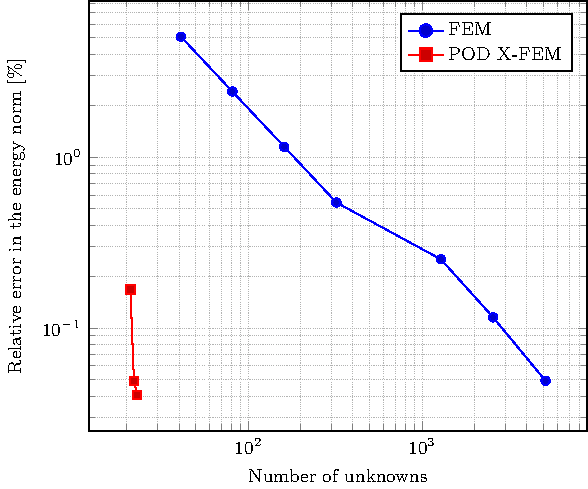
\includegraphics[width=0.45\linewidth]{externals/pgfplots/XFEMNonLinearConvergenceStudy.pdf}}
  \subfigure[Time comparison FEM vs X-PODFEM.]  {\label{fig:TimeNonLinearComparison} 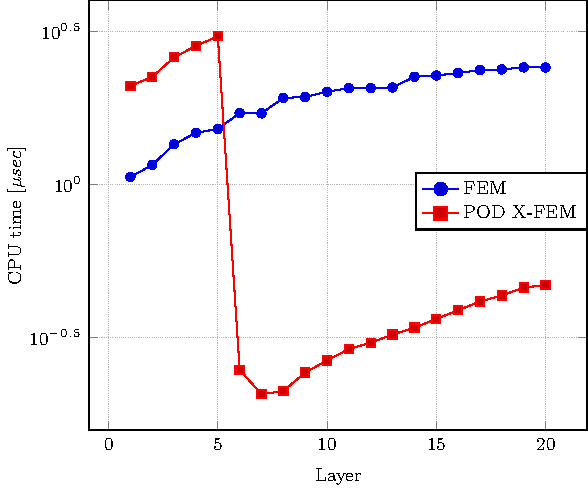
\includegraphics[width=0.45\linewidth]{externals/pgfplots/XFEMNonLinearTimeResults.pdf}}
    \caption{Non-linear problem results}
    \label{NonLinear}
\end{figure}

The PDE of the previous case is modified such that the thermal conductivity $\kappa = \kappa(\theta)$ is now a function of temperature $\theta$. The dependency is obtained smoothing out the thermal conductivity law (given for steel in EUROCODE \cite{EN1993}) by means of a tangent hyperbolic function (see Figure \ref{fig:Conductivity}):
\begin{equation}
	\kappa(\theta) = 54 - 26.7tanh\left(\dfrac{\theta-800}{800}+1\right).
\end{equation}
\begin{figure}[!h]
\centering
  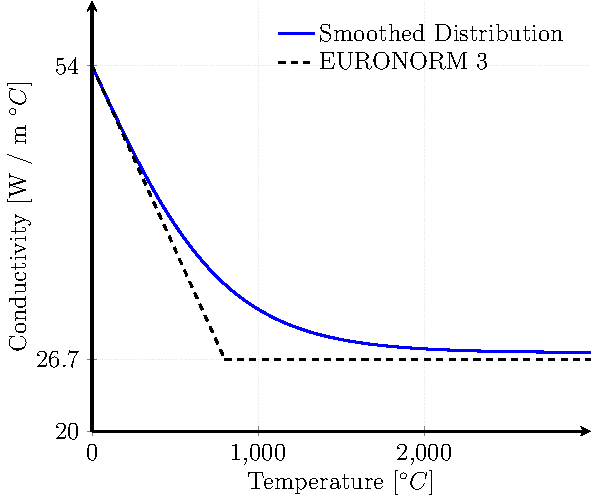
\includegraphics[width=0.5\linewidth]{externals/Pictures/ConductivityDistribution.pdf}
  \caption{Steel conductivity distribution}
  \label{fig:Conductivity}
  
\end{figure}
Figure \ref{fig:NonLinearConvergenceStudy} shows that the same level of accuracy of FEM can be reached using X-PODFEM, but the latter requires much less degrees of freedom (DOFs). In the non-linear case the computational speed-up factor is approximatively 11.1 for the first layers of the ROM-phase, as shown in Figure \ref{fig:TimeNonLinearComparison}. Later, when the computational cost of the coarse mesh dominates, this speed-up will necessarily decrease.

%%%%%%%%%%%%%%%%%%%%%%%%%%%%%%%%%%%%%%%%%%%%%%%%%%%%%%%%%%%%%%%%%%%%%%%%%%%%%%%%%%%%%%%%%%%%%%%%%%%%%%%%%%%%%%%%%%%
% MULTI-PHASE

\subsection*{Non-linear transient heat problem with phase change}
\begin{figure}[!h]
\centering
  \subfigure[Convergence study of the non-linear problem with phase-change.]  {\label{fig:MultiPhaseConvergenceStudy} 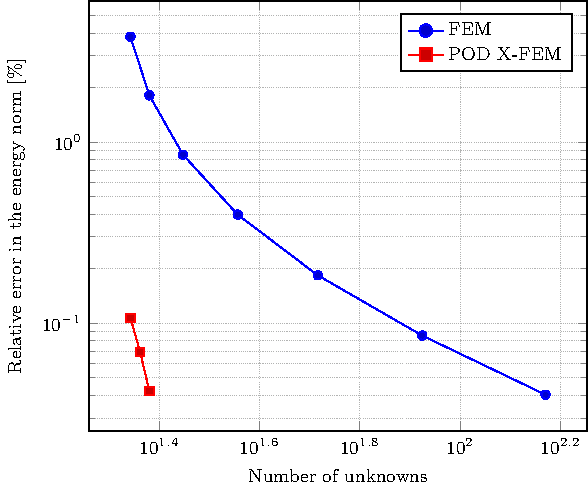
\includegraphics[width=0.45\linewidth]{externals/pgfplots/MultiPhaseXFEMConvergenceStudy.pdf}}
  \subfigure[Time comparison FEM vs X-PODFEM.]  {\label{fig:TimeMultiPhaseComparison} 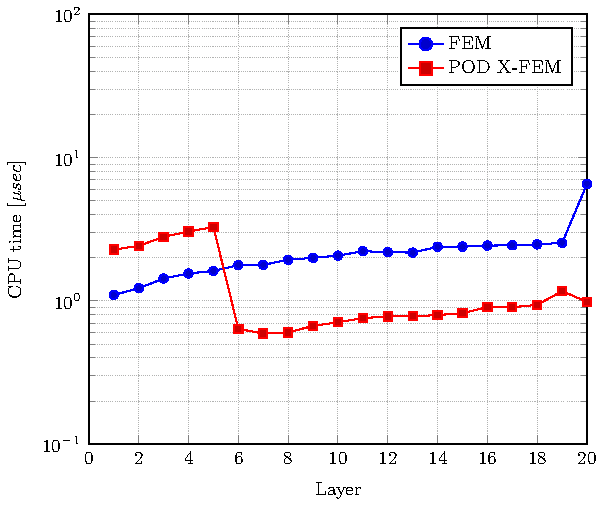
\includegraphics[width=0.45\linewidth]{externals/pgfplots/MultiPhaseTimeResults.pdf}}
    \caption{Multi-phase problem results}
    \label{MultiPhase}
\end{figure}

Finally we want to analyse the behaviour of the method if even the heat capacity term $\rho c = \rho c(\theta)$ is a function of temperature $\theta$.
The heat capacity function is modelled using the temperature-based formulation proposed in \cite{Celentano1994} and depicted in Figure \ref{fig:heatCapacity}:
\begin{equation}
	\rho\c(\theta) = \rho L \dfrac{\partial f_{p}c}{\partial \theta},
\end{equation}
where
\begin{equation}
	\rho\c(\theta) = 
	\begin{cases}
      \dfrac{f^{t+\Delta t}_{pc}-f^{t}_{pc}}{\theta^{t+\Delta t}-\theta^{t}}, & \text{if}\ i\neq 0 \\
      0, & \text{otherwise}
    \end{cases}
\end{equation}

\begin{figure}[!h]
\centering
  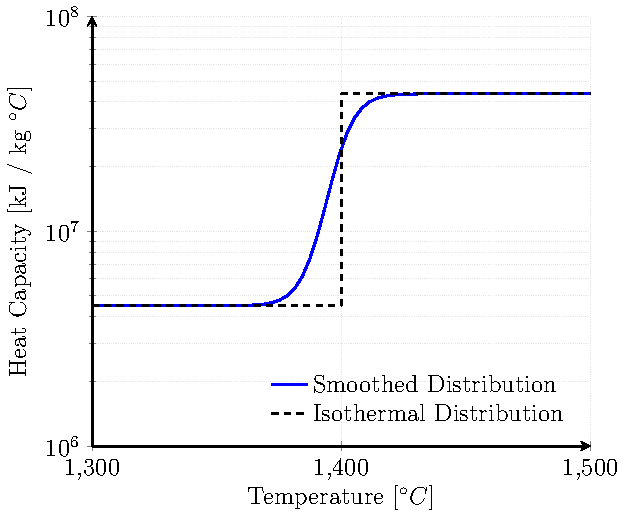
\includegraphics[width=0.5\linewidth]{externals/Pictures/heatCapacity.pdf}
  \caption{Steel heat capacity distribution}
  \label{fig:heatCapacity}
\end{figure}

Figure \ref{fig:MultiPhaseConvergenceStudy} presents the same characteristics of the previous case: 
\begin{itemize}
\item a high level of accuracy can be achieved with a relatively small number of DOFs,
\item increasing the number of POD-modes over-integration is needed in the enriched element.
\end{itemize}
A computational speed-up factor 11.2 is achieved at the beginning of the ROM-phase (Figure \ref{fig:TimeMultiPhaseComparison}).

%%%%%%%%%%%%%%%%%%%%%%%%%%%%%%%%%%%%%%%%%%%%%%%%%%%%%%%%%%%%%%%%%%%%%%%%%%%%%%%%%%%%%%%%%%%%%%%%%%%%%%%%%%%%%%%%%%%
% CONCLUSION 

\section*{Conclusion and further outlooks}
From the results discussed so far we can conclude that the X-PODFEM method, even if applied only to a one-dimensional model, leads to a high accuracy also in case of strongly non-linear problems. Moreover, the method take advantage from the local nature of the AM process in the training-phase, avoiding thus the construction of an artificial \textit{Vademecum}-domain with an eulerian reference frame. In X-PODFEM the construction of the POD-modes is made \textit{on fly} giving higher flexibility in the choice of the training phase and also giving the user the possibility to easily switch, during the same simulation process, from ROM to training-phase.
The computational time required employing X-PODFEM is more than one order of magnitude faster than using FEM with $h$-refinements, we expect that this speed-up will increase even more moving to higher dimensional problems.
 We believe that this results could be also improved employing more sophisticated simulation technologies, e.g. \textit{Isogeometric analysis} (IgA). The use of IgA would lead to a higher accuracy in the results of both the training and the ROM-phase requiring, at the same time, a lower computational effort. The implementation of the method presented in this work together with IgA (X-PODIgA) presents many challenges and it leaves the door open for further outlooks in this direction.   

\bibliographystyle{abbrv}
\bibliography{bibliography.bib}

\end{document}

